\newcommand{\freshResultsAucTable}{
    \begin{center}
        \begin{longtable}[c]{|p{2,8cm}||p{2,8cm} p{2,8cm} p{2,8cm}|}
            \hline
            AUC-ROC & ALOHA & Joint Embedding & Proposed Model \\
            \hline
            \endfirsthead

            \caption*{\raggedright ...continued from previous page} \\
            \hline
            AUC-ROC & ALOHA & Joint Embedding & Proposed Model \\
            \hline
            \endhead

            \caption*{\raggedleft ...continued on next page} \\
            \endfoot

            \caption{Mean and standard deviation AUC-ROC (Area Under Curve) of the different models for the the prediction of the different families on fresh dataset samples. Results were aggregated over \textBF{3} training runs with different weight initializations and minibatch orderings. Best results are shown in \textbf{bold}.} \label{tab:families_aucs}
            \endlastfoot

            Agenttesla & - & \textBF{0.766$\pm$0.051} & 0.608$\pm$0.085 \\
            Avemariarat & - & 0.472$\pm$0.064 & \textBF{0.529$\pm$0.049} \\
            Azorult & - & \textBF{0.624$\pm$0.018} & 0.601$\pm$0.031 \\
            Formbook & - & \textBF{0.588$\pm$0.007} & 0.526$\pm$0.023 \\
            Heodo & - & \textBF{0.853$\pm$0.008} & 0.770$\pm$0.012 \\
            Loki & - & \textBF{0.597$\pm$0.031} & 0.568$\pm$0.026 \\
            Masslogger & - & \textBF{0.564$\pm$0.018} & 0.562$\pm$0.022 \\
            Netwire & - & 0.463$\pm$0.030 & \textBF{0.538$\pm$0.033} \\
            Njrat & - & \textBF{0.757$\pm$0.001} & 0.732$\pm$0.018 \\
            Remcorsat & - & 0.482$\pm$0.033 & \textBF{0.549$\pm$0.049} \\
            \hline
        \end{longtable}
    \end{center}
}

\newcommand{\freshResultsSummaryTable}{
    \begin{center}
        \begin{longtable}[c]{|p{3,2cm}||p{1,8cm} p{1,8cm} p{1,8cm} p{1,8cm} p{1,8cm}|}
            \hline
            & TPR & Accuracy & Precision & Recall & F1 score \\
            \hline
            \endfirsthead

            \caption*{\raggedright ...continued from previous page} \\
            \hline
            & TPR & Accuracy & Precision & Recall & F1 score \\
            \hline
            \endhead

            \caption*{\raggedleft ...continued on next page} \\
            \endfoot

            \caption{Summary of the mean and standard deviation results of the different models for the prediction of the different families on fresh dataset samples at \textbf{FPR} $=1\%$. Results were aggregated over \textBF{3} training runs with different weight initializations and minibatch orderings. Best results are shown in \textbf{bold}.} \label{tab:fresh_results_summary}
            \endlastfoot

            \multicolumn{6}{|c|}{\textbf{Agenttesla} (at FPR $=1\%$)} \\
            \hline
            Joint Embedding & \textBF{0.034$\pm$0.004} & \textBF{0.900$\pm$0.000} & \textBF{1.000$\pm$0.000} & \textBF{0.000$\pm$0.000} & \textBF{0.000$\pm$0.000} \\
            Proposed Model & 0.018$\pm$0.006 & \textBF{0.900$\pm$0.000} & \textBF{1.000$\pm$0.000} & \textBF{0.000$\pm$0.000} & \textBF{0.000$\pm$0.000} \\
            \hline
            \multicolumn{6}{|c|}{\textbf{Avemariarat} (at FPR $=1\%$)} \\
            \hline
            Joint Embedding & 0.012$\pm$0.004 & \textBF{0.900$\pm$0.000} & \textBF{1.000$\pm$0.000} & \textBF{0.000$\pm$0.000} & \textBF{0.000$\pm$0.000} \\
            Proposed Model & \textBF{0.012$\pm$0.003} & \textBF{0.900$\pm$0.000} & \textBF{1.000$\pm$0.000} & \textBF{0.000$\pm$0.000} & \textBF{0.000$\pm$0.000} \\
            \hline
            \multicolumn{6}{|c|}{\textbf{Azorult} (at FPR $=1\%$)} \\
            \hline
            Joint Embedding & \textBF{0.017$\pm$0.002} & \textBF{0.900$\pm$0.000} & \textBF{1.000$\pm$0.000} & \textBF{0.000$\pm$0.000} & \textBF{0.000$\pm$0.000} \\
            Proposed Model & 0.015$\pm$0.001 & \textBF{0.900$\pm$0.000} & \textBF{1.000$\pm$0.000} & \textBF{0.000$\pm$0.000} & \textBF{0.000$\pm$0.000} \\
            \hline
            \multicolumn{6}{|c|}{\textbf{Formbook} (at FPR $=1\%$)} \\
            \hline
            Joint Embedding & \textBF{0.016$\pm$0.001} & \textBF{0.900$\pm$0.000} & \textBF{1.000$\pm$0.000} & \textBF{0.000$\pm$0.000} & \textBF{0.000$\pm$0.000} \\
            Proposed Model & 0.011$\pm$0.001 & \textBF{0.900$\pm$0.000} & \textBF{1.000$\pm$0.000} & \textBF{0.000$\pm$0.000} & \textBF{0.000$\pm$0.000} \\
            \hline
            \multicolumn{6}{|c|}{\textbf{Heodo} (at FPR $=1\%$)} \\
            \hline
            Joint Embedding & \textBF{0.045$\pm$0.004} & \textBF{0.900$\pm$0.000} & \textBF{1.000$\pm$0.000} & \textBF{0.000$\pm$0.000} & \textBF{0.000$\pm$0.000} \\
            Proposed Model & 0.028$\pm$0.003 & \textBF{0.900$\pm$0.000} & \textBF{1.000$\pm$0.000} & \textBF{0.000$\pm$0.000} & \textBF{0.000$\pm$0.000} \\
            \hline
            \multicolumn{6}{|c|}{\textbf{Loki} (at FPR $=1\%$)} \\
            \hline
            Joint Embedding & 0.013$\pm$0.002 & \textBF{0.900$\pm$0.000} & \textBF{1.000$\pm$0.000} & \textBF{0.000$\pm$0.000} & \textBF{0.000$\pm$0.000} \\
            Proposed Model & \textBF{0.013$\pm$0.001} & \textBF{0.900$\pm$0.000} & \textBF{1.000$\pm$0.000} & \textBF{0.000$\pm$0.000} & \textBF{0.000$\pm$0.000} \\
            \hline
            \multicolumn{6}{|c|}{\textbf{Masslogger} (at FPR $=1\%$)} \\
            \hline
            Joint Embedding & \textBF{0.018$\pm$0.003} & \textBF{0.900$\pm$0.000} & \textBF{1.000$\pm$0.000} & \textBF{0.000$\pm$0.000} & \textBF{0.000$\pm$0.000} \\
            Proposed Model & 0.013$\pm$0.001 & \textBF{0.900$\pm$0.000} & \textBF{1.000$\pm$0.000} & \textBF{0.000$\pm$0.000} & \textBF{0.000$\pm$0.000} \\
            \hline
            \multicolumn{6}{|c|}{\textbf{Netwire} (at FPR $=1\%$)} \\
            \hline
            Joint Embedding & 0.010$\pm$0.002 & \textBF{0.900$\pm$0.000} & \textBF{1.000$\pm$0.000} & \textBF{0.000$\pm$0.000} & \textBF{0.000$\pm$0.000} \\
            Proposed Model & \textBF{0.013$\pm$0.003} & \textBF{0.900$\pm$0.000} & \textBF{1.000$\pm$0.000} & \textBF{0.000$\pm$0.000} & \textBF{0.000$\pm$0.000} \\
            \hline
            \multicolumn{6}{|c|}{\textbf{Njrat} (at FPR $=1\%$)} \\
            \hline
            Joint Embedding & \textBF{0.040$\pm$0.003} & \textBF{0.900$\pm$0.000} & \textBF{1.000$\pm$0.000} & \textBF{0.000$\pm$0.000} & \textBF{0.000$\pm$0.000} \\
            Proposed Model & 0.028$\pm$0.003 & \textBF{0.900$\pm$0.000} & \textBF{1.000$\pm$0.000} & \textBF{0.000$\pm$0.000} & \textBF{0.000$\pm$0.000} \\
            \hline
            \multicolumn{6}{|c|}{\textbf{Remcorsat} (at FPR $=1\%$)} \\
            \hline
            Joint Embedding & 0.010$\pm$0.003 & \textBF{0.900$\pm$0.000} & \textBF{1.000$\pm$0.000} & \textBF{0.000$\pm$0.000} & \textBF{0.000$\pm$0.000} \\
            Proposed Model & \textBF{0.012$\pm$0.002} & \textBF{0.900$\pm$0.000} & \textBF{1.000$\pm$0.000} & \textBF{0.000$\pm$0.000} & \textBF{0.000$\pm$0.000} \\
            \hline
        \end{longtable}
    \end{center}
}

\newcommand{\allMeanFreshRocJointEmbedding}{
    \begin{figure}[H]
        \vspace*{-0.5cm}
        \centering
        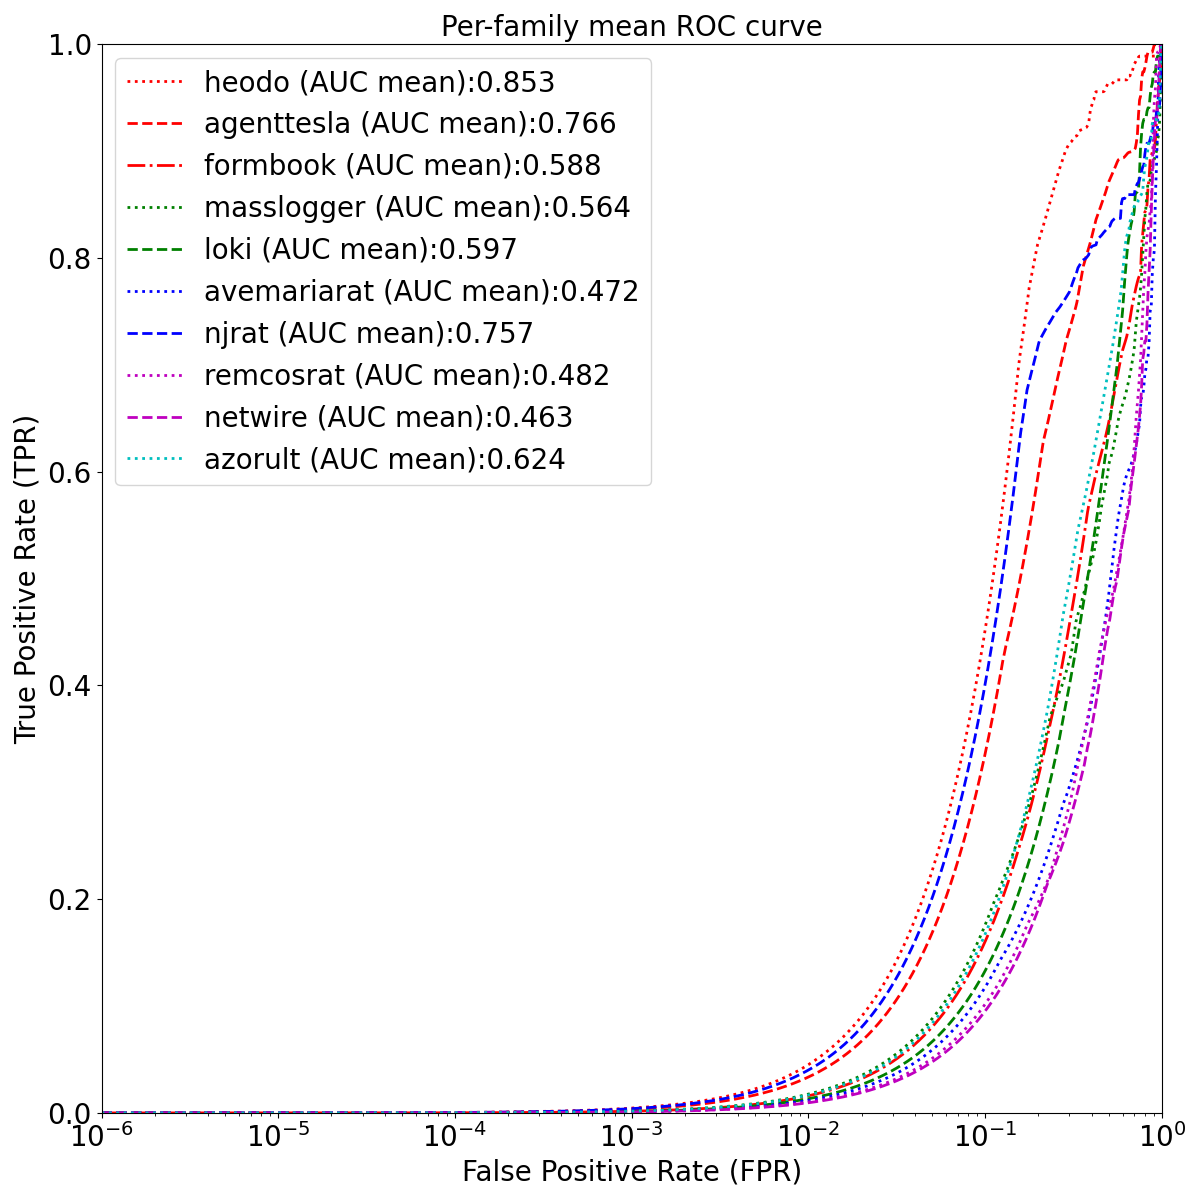
\includegraphics[width=0.6\textwidth]{./results/all_mean_fresh_roc_jointEmbedding.png}
        \vspace*{-0.2cm}
        \caption{Mean ROC curve and AUC statistics of \textBF{Joint Embedding} model for the prediction of all families on fresh dataset samples. The line represents the \textit{mean} TPR at a given FPR. Statistics were computed over \textBF{3} training runs, each with random parameter initialization.}
        \label{fig:allMeanFreshRocJointEmbedding}
    \end{figure}
}

\newcommand{\allMeanFreshRocProposedModel}{
    \begin{figure}[H]
        \vspace*{-0.5cm}
        \centering
        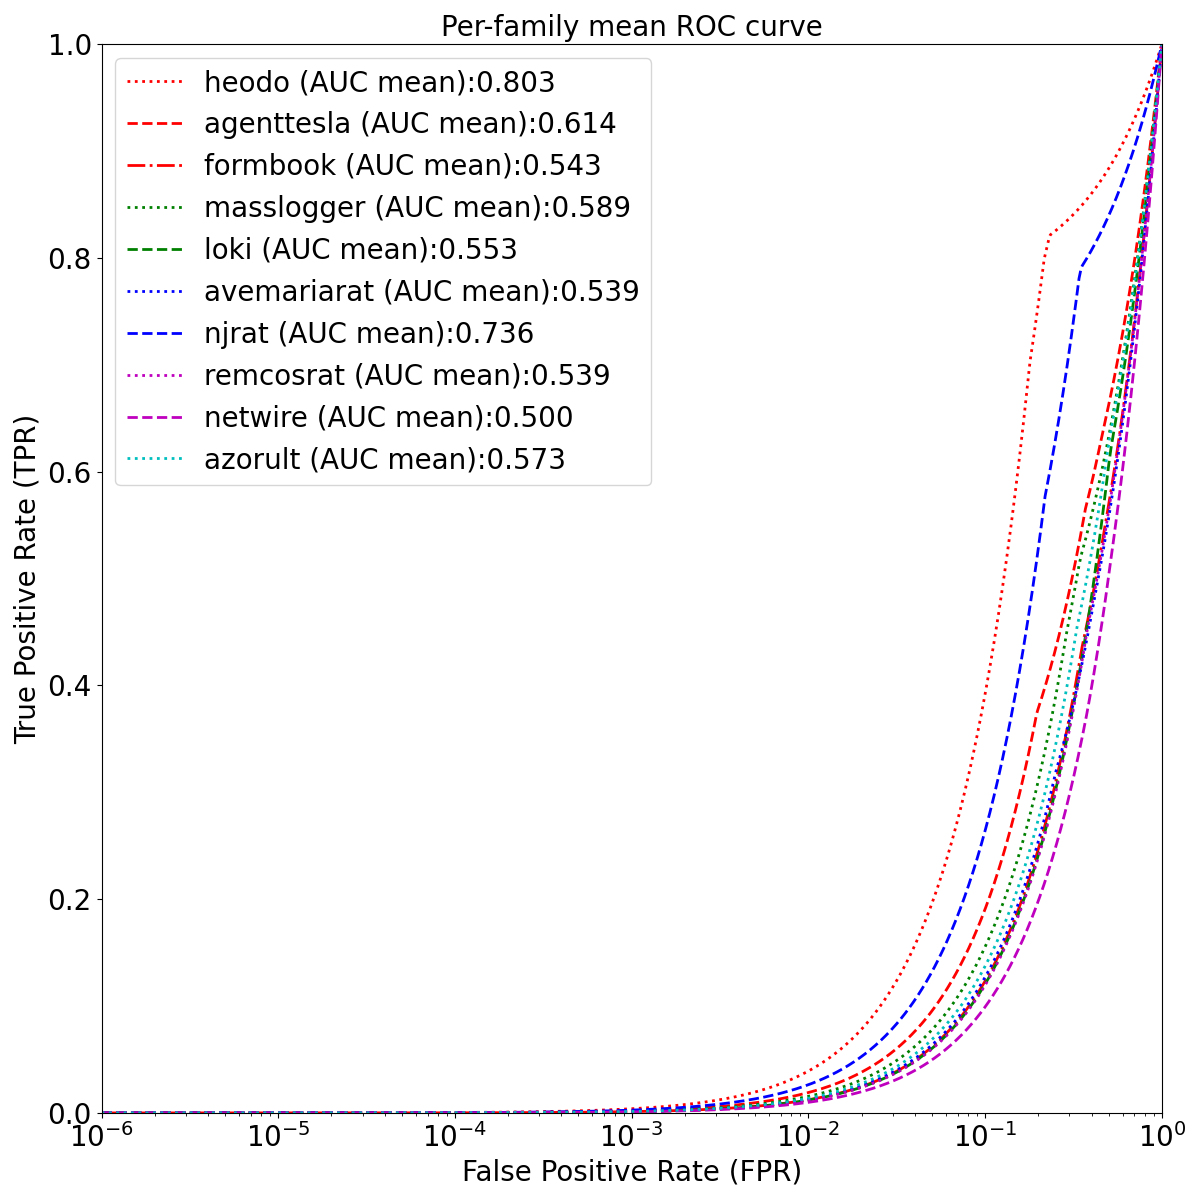
\includegraphics[width=0.6\textwidth]{./results/all_mean_fresh_roc_proposedModel.png}
        \vspace*{-0.2cm}
        \caption{Mean ROC curve and AUC statistics of \textBF{Proposed Model} for the prediction of all families on fresh dataset samples. The line represents the \textit{mean} TPR at a given FPR. Statistics were computed over \textBF{3} training runs, each with random parameter initialization.}
        \label{fig:allMeanFreshRocProposedModel}
    \end{figure}
}